\section{Anime Dataset}

{\bf Attributes:} Rank, Name, Japanese\_name, Type, Episodes, Studio, Release\_season, Tags, Rating, Release\_year, End\_year, Description, Content\_Warning, Related\_Mange, Related\_anime, Voice\_actors, staff\\

{\bf Scenario:}  A streaming service is considering expanding its short anime series catalog ($<$ 25 episodes) and wants to understand how viewer ratings differ between anime TV series and movies released after 2015. The goal is to determine which format generally receives better audience reception to inform licensing and promotion strategies.\\

{\bf Research Question:} How do audience ratings compare between anime TV series and movies released after 2015, and which format generally receives higher ratings?

\subsection{Part A: Data Cleaning and Preprocessing}
First, filter your dataset so that only the variables critical for your analysis remain. Then clean your data so that there is consistency in variable types, capitalization, and handle any missing or invalid values.\\
-----\\
We first filtered by Year to keep everything released after 2015, then removed all of the columns irrelevant to the research question, leaving 'Type' and 'Rating'. After doing a drop of all rows with missing values and renaming the columns so they are consistent to how the albums data was set up, there was much whitespace left in the attribute values of the type column, so that was stripped away. \\

At that point we could force all of the type values to lowercase and read out a dictionary to ensure that there were not any misspelling concerns. Below is the corresponding utility function:\\
 
\begin{verbatim}
def clean_preprocess_anime_data(input_csv: str, output_csv: str) -> pd.DataFrame:
    """
    Cleans and preprocesses the anime dataset by filtering out the irrelevant features
    and datapoints and reformatting the columns names and attribute values

    :param input_csv:: Path to the input CSV file containing the anime dataset.
    :type input_csv: str
    :param output_csv: Filename for the clean data.
    :type output_csv: str
    :returns: pd.DataFrame
    :rtype: pd.DataFrame
    """
    df = pd.read_csv(input_csv)

    # Keeps relevant variables, relevant data poitns, removes the
    # missing value rows, renames the columns, and strips the whitespace
    # out for the type col
    df = df[df['Release_year'] > 2015]
    df = df.loc[:, ['Type', 'Rating']]
    df.dropna(inplace=True)
    df.columns = ['type', 'rating']
    df['type'] = df['type'].str.strip()

    # Standardizes to lower case and filters out irrelevant types
    df['type'] = df['type'].str.lower()
    df = df[df['type'].isin(['tv', 'movie'])]
    print(df['type'].value_counts().to_dict())

    os.makedirs(f'../datasets/clean/', exist_ok=True)
    df.to_csv(f'../datasets/clean/{output_csv}', index=False)
    return df
\end{verbatim}

\begin{center}
\textbf{Figure 6:} Anime data pre-processing function.
\end{center}

Below is a comparison for this dataset to illustrate the changes:\\

\noindent\textbf{Anime.csv}
\begin{verbatim}
Rank,Name,Japanese_name,Type,Episodes,Studio,Release_season,Tags,Rating,Release_year,End_year,Description,Content_Warning,Related_Mange,Related_anime,Voice_actors,staff
1,Demon Slayer: Kimetsu no Yaiba - Entertainment District Arc, Kimetsu no Yaiba: Yuukaku-hen,TV   ,,ufotable,Fall ,"Action, Adventure, Fantasy, Shounen, Demons, Historical, Martial Arts, Orphans, Siblings, Swordplay, Based on a Manga, Explicit Violence",4.6,2021.0,,"'Tanjiro and his friends accompany the Hashira Tengen Uzui to an entertainment district where Tengen’s female ninja agents were gathering information on a demon before they suddenly disappeared. In order to investigate, Tanjiro and the others disguise themselves as women to sneak in!'",Explicit Violence,Demon Slayer: Kimetsu no Yaiba,"Demon Slayer: Kimetsu no Yaiba, Demon Slayer: Kimetsu no Yaiba Movie - Mugen Train, Demon Slayer: Kimetsu no Yaiba - Mugen Train","Inosuke Hashibira : Yoshitsugu Matsuoka, Nezuko Kamado : Akari Kitou, Tanjirou Kamado : Natsuki Hanae, Zenitsu Agatsuma : Hiro Shimono, Daki : Miyuki Sawashiro, Tengen Uzui : Katsuyuki Konishi, Akaza : Akira Ishida, Amane Ubuyashiki, Koyoharu Gotouge
Original Creator, Haruo Sotozaki
Director, Akira Matsushima
Character Design, Aimer
Song Performance","Koyoharu Gotouge : Original Creator, Haruo Sotozaki : Director, Akira Matsushima : Character Design, Aimer : Song Performance"
2,Fruits Basket the Final Season, Fruits Basket the Final,TV   ,13.0,TMS Entertainment,Spring,"Drama, Fantasy, Romance, Shoujo, Animal Transformation, Contemporary Fantasy, Curse, Dysfunctional Families, Mental Illness, Orphans, Based on a Manga, Emotional Abuse,, Mature Themes,, Physical Abuse,, Suicide,, Violence,, Domestic Abuse",4.6,2021.0,,'The final arc of Fruits Basket.',"Emotional Abuse,, Mature Themes,, Physical Abuse,, Suicide,, Violence,, Domestic Abuse","Fruits Basket, Fruits Basket Another","Fruits Basket 1st Season, Fruits Basket 2nd Season","Akito Sohma : Maaya Sakamoto, Kyo Sohma : Yuuma Uchida, Shigure Sohma : Yuuichi Nakamura, Tohru Honda : Manaka Iwami, Yuki Sohma : Nobunaga Shimazaki, Arisa Uotani : Atsumi Tanezaki, Hatsuharu Sohma : Makoto Furukawa, Isuzu Sohma : Aki Toyosaki, Natsuki Takaya
Original Creator, Yoshihide Ibata
Director & Episode Director & Storyboard, Taku Kishimoto
Screenplay & Series Composition, Masaru Yokoyama
Music, Masaru Shindou
Character Design & Chief Animation Director, Baek-Ryun Chae
Photography Director, Youko Koyama
Art Director, Mika Sugawara
Color Design","Natsuki Takaya : Original Creator, Yoshihide Ibata : Director & Episode Director & Storyboard, Taku Kishimoto : Screenplay & Series Composition, Masaru Yokoyama : Music, Masaru Shindou : Character Design & Chief Animation Director, Baek-Ryun Chae : Photography Director, Youko Koyama : Art Director, Mika Sugawara : Color Design"
3,Mo Dao Zu Shi 3, The Founder of Diabolism 3,Web  ,12.0,B.C MAY PICTURES,,"Fantasy, Ancient China, Chinese Animation, Cultivation, Xianxia, Based on a Web Novel",4.58,2021.0,,'The third season of Mo Dao Zu Shi.',,"Grandmaster of Demonic Cultivation: Mo Dao Zu Shi (Novel), The Master of Diabolism","Mo Dao Zu Shi 2, Mo Dao Zu Shi Q","Lan Wangji, Wei Wuxian, Jiang Cheng, Jin Guangyao, Jin Ling, Lan Jingyi, Lan Sizhui, Lan Xichen, Mo Xiang Tong Xiu
Original Creator, Xiong Ke
Chief Director, Ma Chendi
Chief Director, Sun Yujing
Music, Weng Teng
Music, Feng Shuo
Music, Shen Lin
Character Design & Chief Animation Director, Liang Sha
Screenplay","Mo Xiang Tong Xiu : Original Creator, Xiong Ke : Chief Director, Ma Chendi : Chief Director, Sun Yujing : Music, Weng Teng : Music, Feng Shuo : Music, Shen Lin : Character Design & Chief Animation Director, Liang Sha : Screenplay"
4,Fullmetal Alchemist: Brotherhood, Hagane no Renkinjutsushi: Full Metal Alchemist,TV   ,64.0,Bones,Spring,"Action, Adventure, Drama, Fantasy, Mystery, Shounen, Conspiracy, Death of a Loved One, Military, Siblings, Based on a Manga, Animal Abuse,, Mature Themes,, Violence,, Domestic Abuse",4.58,2009.0,2010.0,"""The foundation of alchemy is based on the law of equivalent exchange; you cannot produce something from nothing. As such, alchemy is bound by one taboo - human transmutation. Four years ago two young brothers, Edward and Alphonse Elric, broke this taboo when they tried to resurrect their dead mother. During the process Al's body disintegrated and Ed lost his leg. In a desperate attempt to prevent his brother from disappearing completely, Ed sacrificed one of his arms so he could affix Al's soul to a suit of armor. When his missing limbs are replaced by auto mail parts, Ed bears the name of the Fullmetal Alchemist - the youngest ever State Alchemist and dog of the military. Now, alongside his brother, Ed uses his status within the military to attempt to find any way that he can return their bodies back to their original state.""","Animal Abuse,, Mature Themes,, Violence,, Domestic Abuse","Fullmetal Alchemist, Fullmetal Alchemist (Light Novel), Fullmetal Alchemist Gaiden, Fullmetal Alchemist: The Prototype, Fullmetal Alchemist: The Complete Four-Panel Comics","Fullmetal Alchemist: Brotherhood Specials, Fullmetal Alchemist: Brotherhood: 4-Koma Theater, Fullmetal Alchemist: The Sacred Star of Milos","Alphonse Elric : Rie Kugimiya, Edward Elric : Romi Park, Alex Louis Armstrong : Kenji Utsumi, Barry The Chopper : Hideyuki Umezu, Buccaneer : Ryuzaburo Otomo, Darius : Masuo Amada, Envy : Minami Takayama, Father : Iemasa Kayumi, Hiromu Arakawa
Original Creator, Yasuhiro Irie
Director, Akira Senju
Music, Hiroki Kanno
2Nd Key Animator & Animation Director & Assistant Animation Director & Character Design & Key Animator, Hiroo Maruyama
Producer, Ryou Ooyama
Producer, Nobuyuki Kurashige
Producer, Noritomo Yonai
Producer","Hiromu Arakawa : Original Creator, Yasuhiro Irie : Director, Akira Senju : Music, Hiroki Kanno : 2Nd Key Animator & Animation Director & Assistant Animation Director & Character Design & Key Animator, Hiroo Maruyama : Producer, Ryou Ooyama : Producer, Nobuyuki Kurashige : Producer, Noritomo Yonai : Producer"
5,Attack on Titan 3rd Season: Part II, Shingeki no Kyojin Season 3: Part II,TV   ,10.0,WIT Studio,Spring,"Action, Fantasy, Horror, Shounen, Dark Fantasy, Isolated Society, Military, Outside World, Post-apocalyptic, Based on a Manga, Cannibalism,, Explicit Violence",4.57,2019.0,,"'The battle to retake Wall Maria begins now! With Eren’s new hardening ability, the Scouts are confident they can seal the wall and take back Shiganshina District. If they succeed, Eren can finally unlock the secrets of the basement—and the world. But danger lies in wait as Reiner, Bertholdt, and the Beast Titan have plans of their own. Could this be humanity’s final battle for survival?'","Cannibalism,, Explicit Violence","Attack on Titan, Attack on Titan: End of the World (Light Novel)","Attack on Titan, Attack on Titan 2nd Season, Attack on Titan 3rd Season, Attack on Titan 3rd Season: Part II Specials, Attack on Titan Movie 4: Chronicle, Attack on Titan The Final Season, Attack on Titan The Final Season: Part II","Armin Arlelt : Marina Inoue, Eren Jaeger : Yuuki Kaji, Mikasa Ackerman : Yui Ishikawa, Armored Titan, Beast Titan : Takehito Koyasu, Bertholdt Hoover : Tomohisa Hashizume, Erwin Smith : Daisuke Ono, Hange Zoe : Romi Park, Hajime Isayama
Original Creator, Tetsurou Araki
Chief Director, Masashi Koizuka
Director, Tetsuya Wakano
Assistant Director, Yasuko Kobayashi
Series Composition, Hiroyuki Sawano
Music, Kyouji Asano
Character Design, Kazuhiro Yamada
Photography Director","Hajime Isayama : Original Creator, Tetsurou Araki : Chief Director, Masashi Koizuka : Director, Tetsuya Wakano : Assistant Director, Yasuko Kobayashi : Series Composition, Hiroyuki Sawano : Music, Kyouji Asano : Character Design, Kazuhiro Yamada : Photography Director"
...
\end{verbatim}

\noindent\textbf{anime.csv}
\begin{verbatim}
type,rating
tv,4.6
tv,4.6
tv,4.57
tv,4.56
tv,4.56
...
\end{verbatim}

\begin{center}
    \textbf{Figure 7:} Raw vs. Cleaned Anime dataset.
\end{center}
\newpage

\subsection{Part B: Generate Three Visualizations}
Produce the following types of plots:
\begin{itemize}
    \item \textbf{Error Bar Plot:} Show the mean and variability (e.g., standard error or 95\% confidence intervals) of the numerical variable across each category.
    \item \textbf{Barcode Chart:} Also known as a strip plot or rug plot. Shows individual data points across categories.
    \item \textbf{Histogram:} Plot the distribution of the numerical variable, grouped by the categorical variable (using hue or facet).
\end{itemize}
-----\\
\textbf{Error Bar Plot}
\begin{center}
  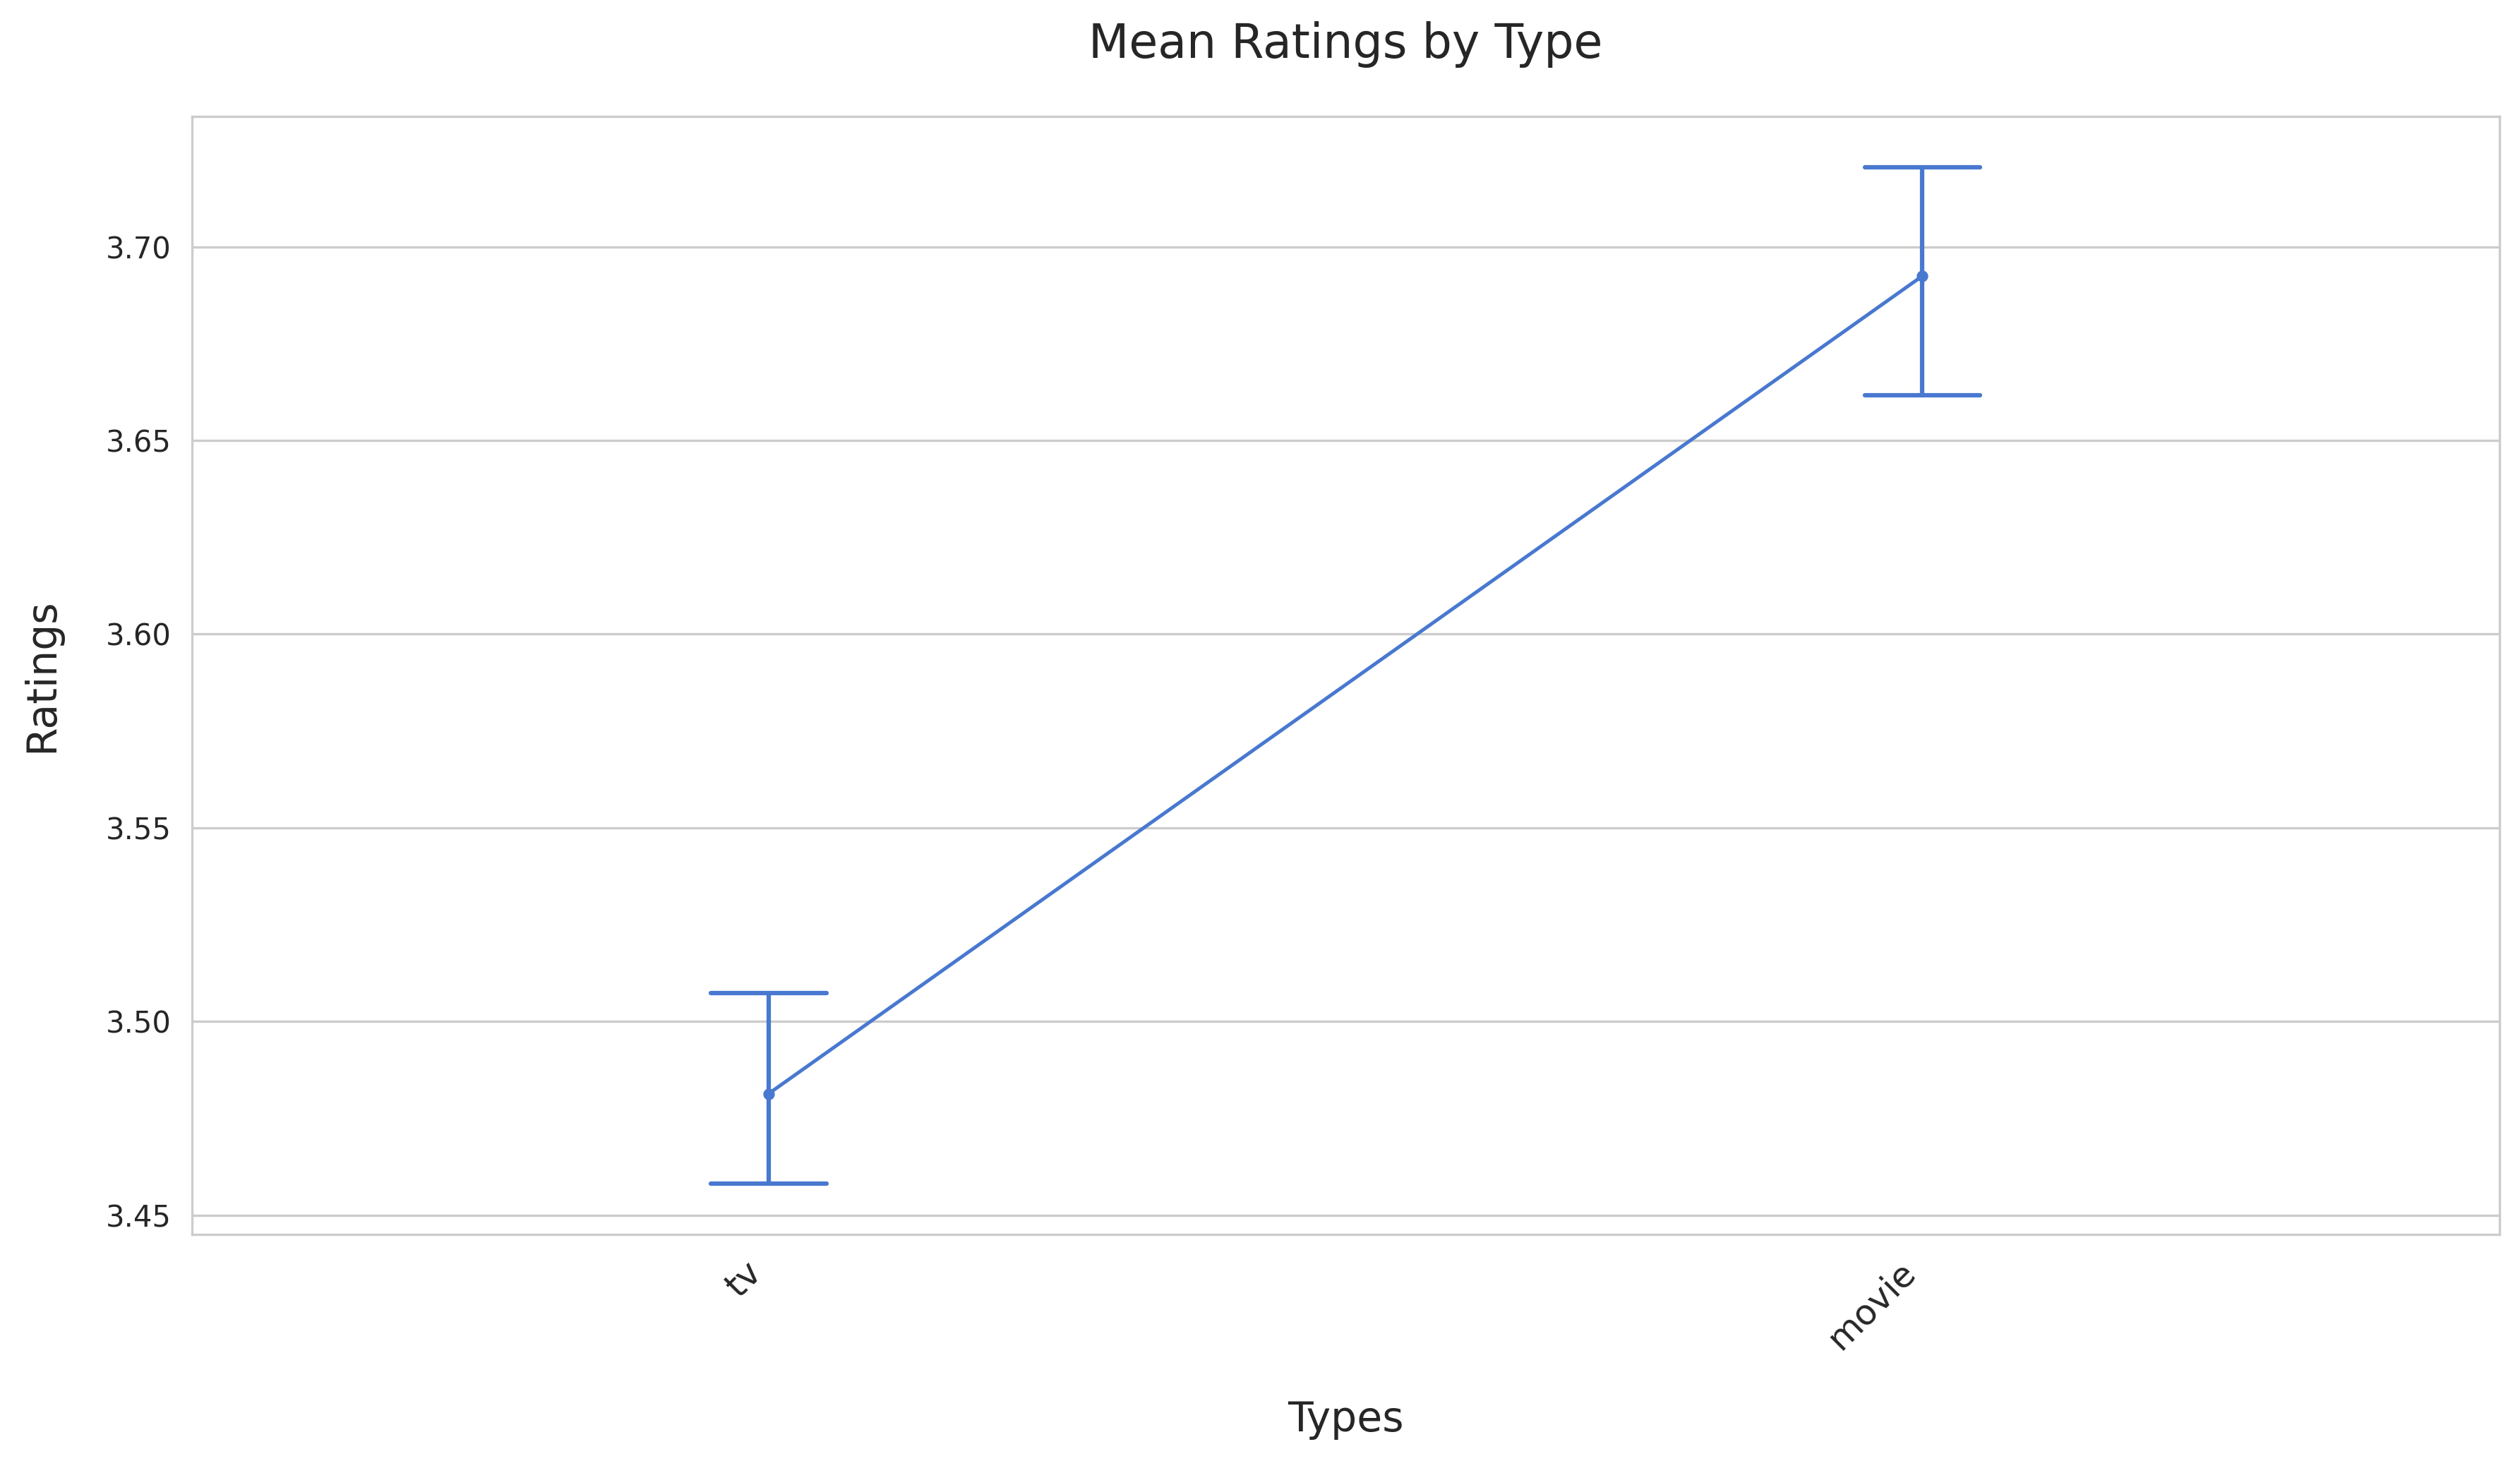
\includegraphics[width=0.95\textwidth]{figures/ratings_by_type_error_bar_plot.png}
  
  \textbf{Figure 8:} Mean Ratings by Type with 95\% confidence intervals.
\end{center}

\textbf{Barcode Chart}
\begin{center}
  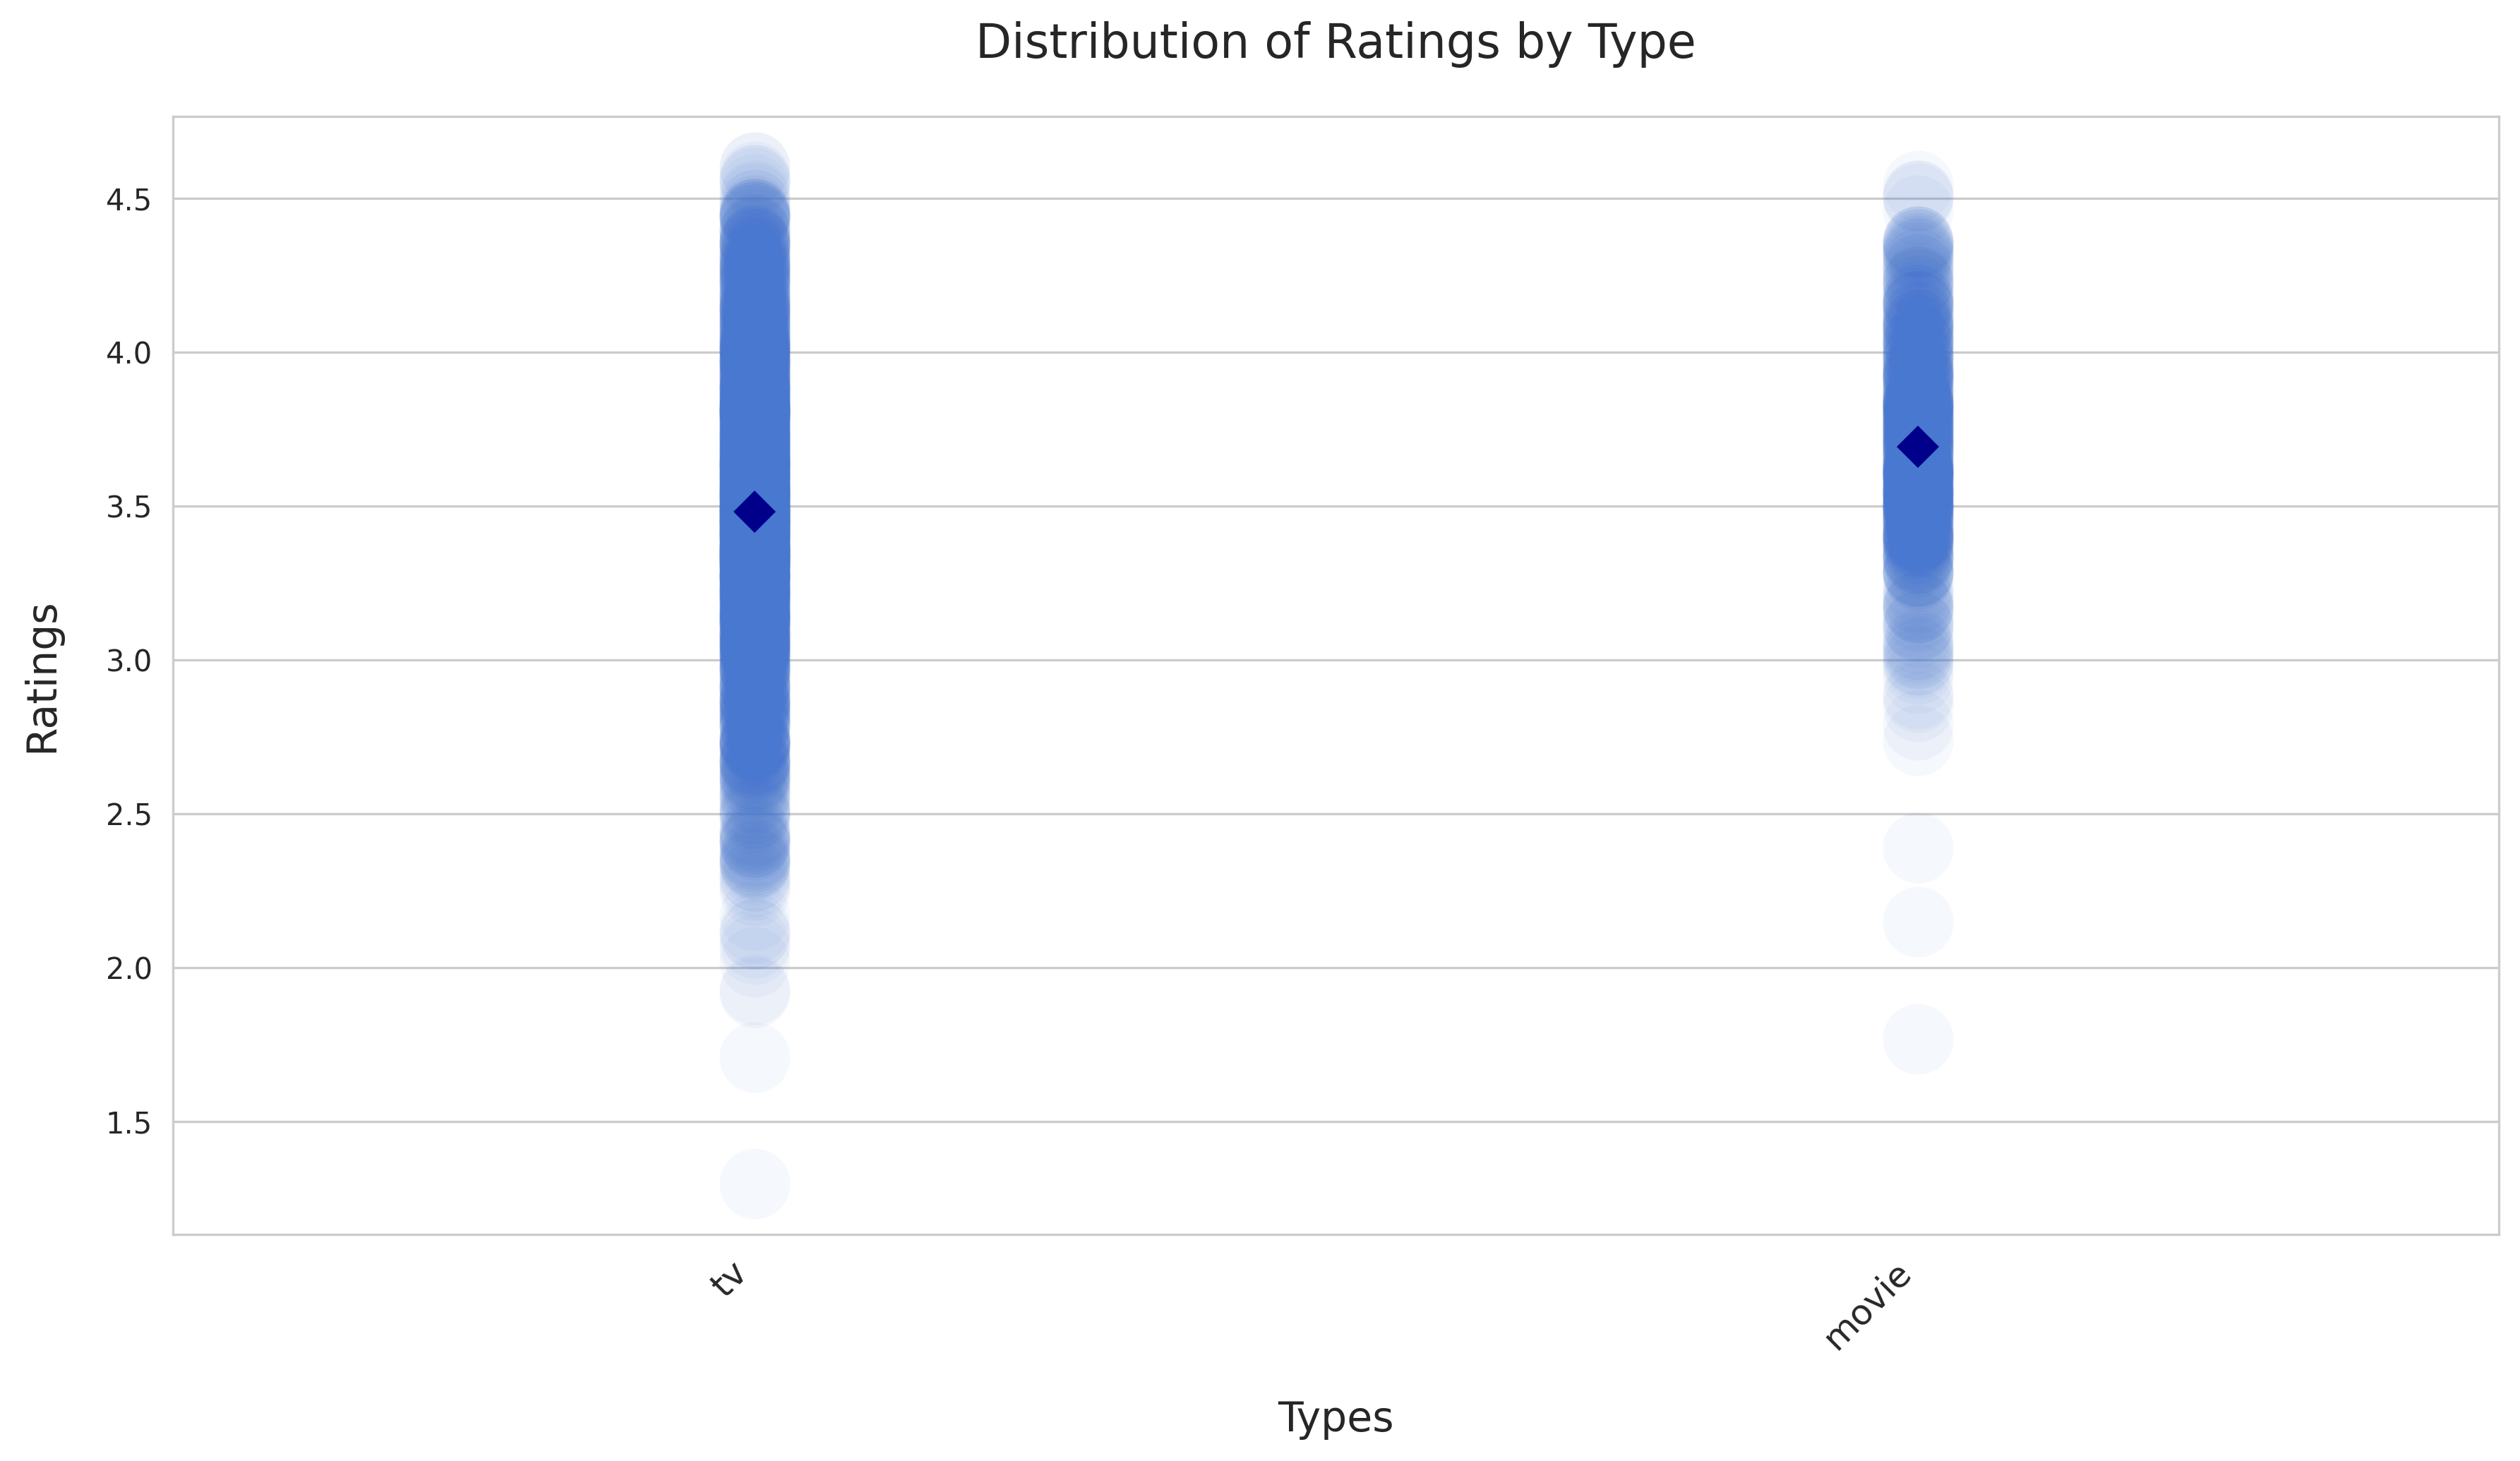
\includegraphics[width=0.95\textwidth]{figures/ratings_by_type_strip_plot.png}
  
  \textbf{Figure 9:} Average Distribution of Ratings by Type.
\end{center}

\textbf{Histogram}
\begin{center}
  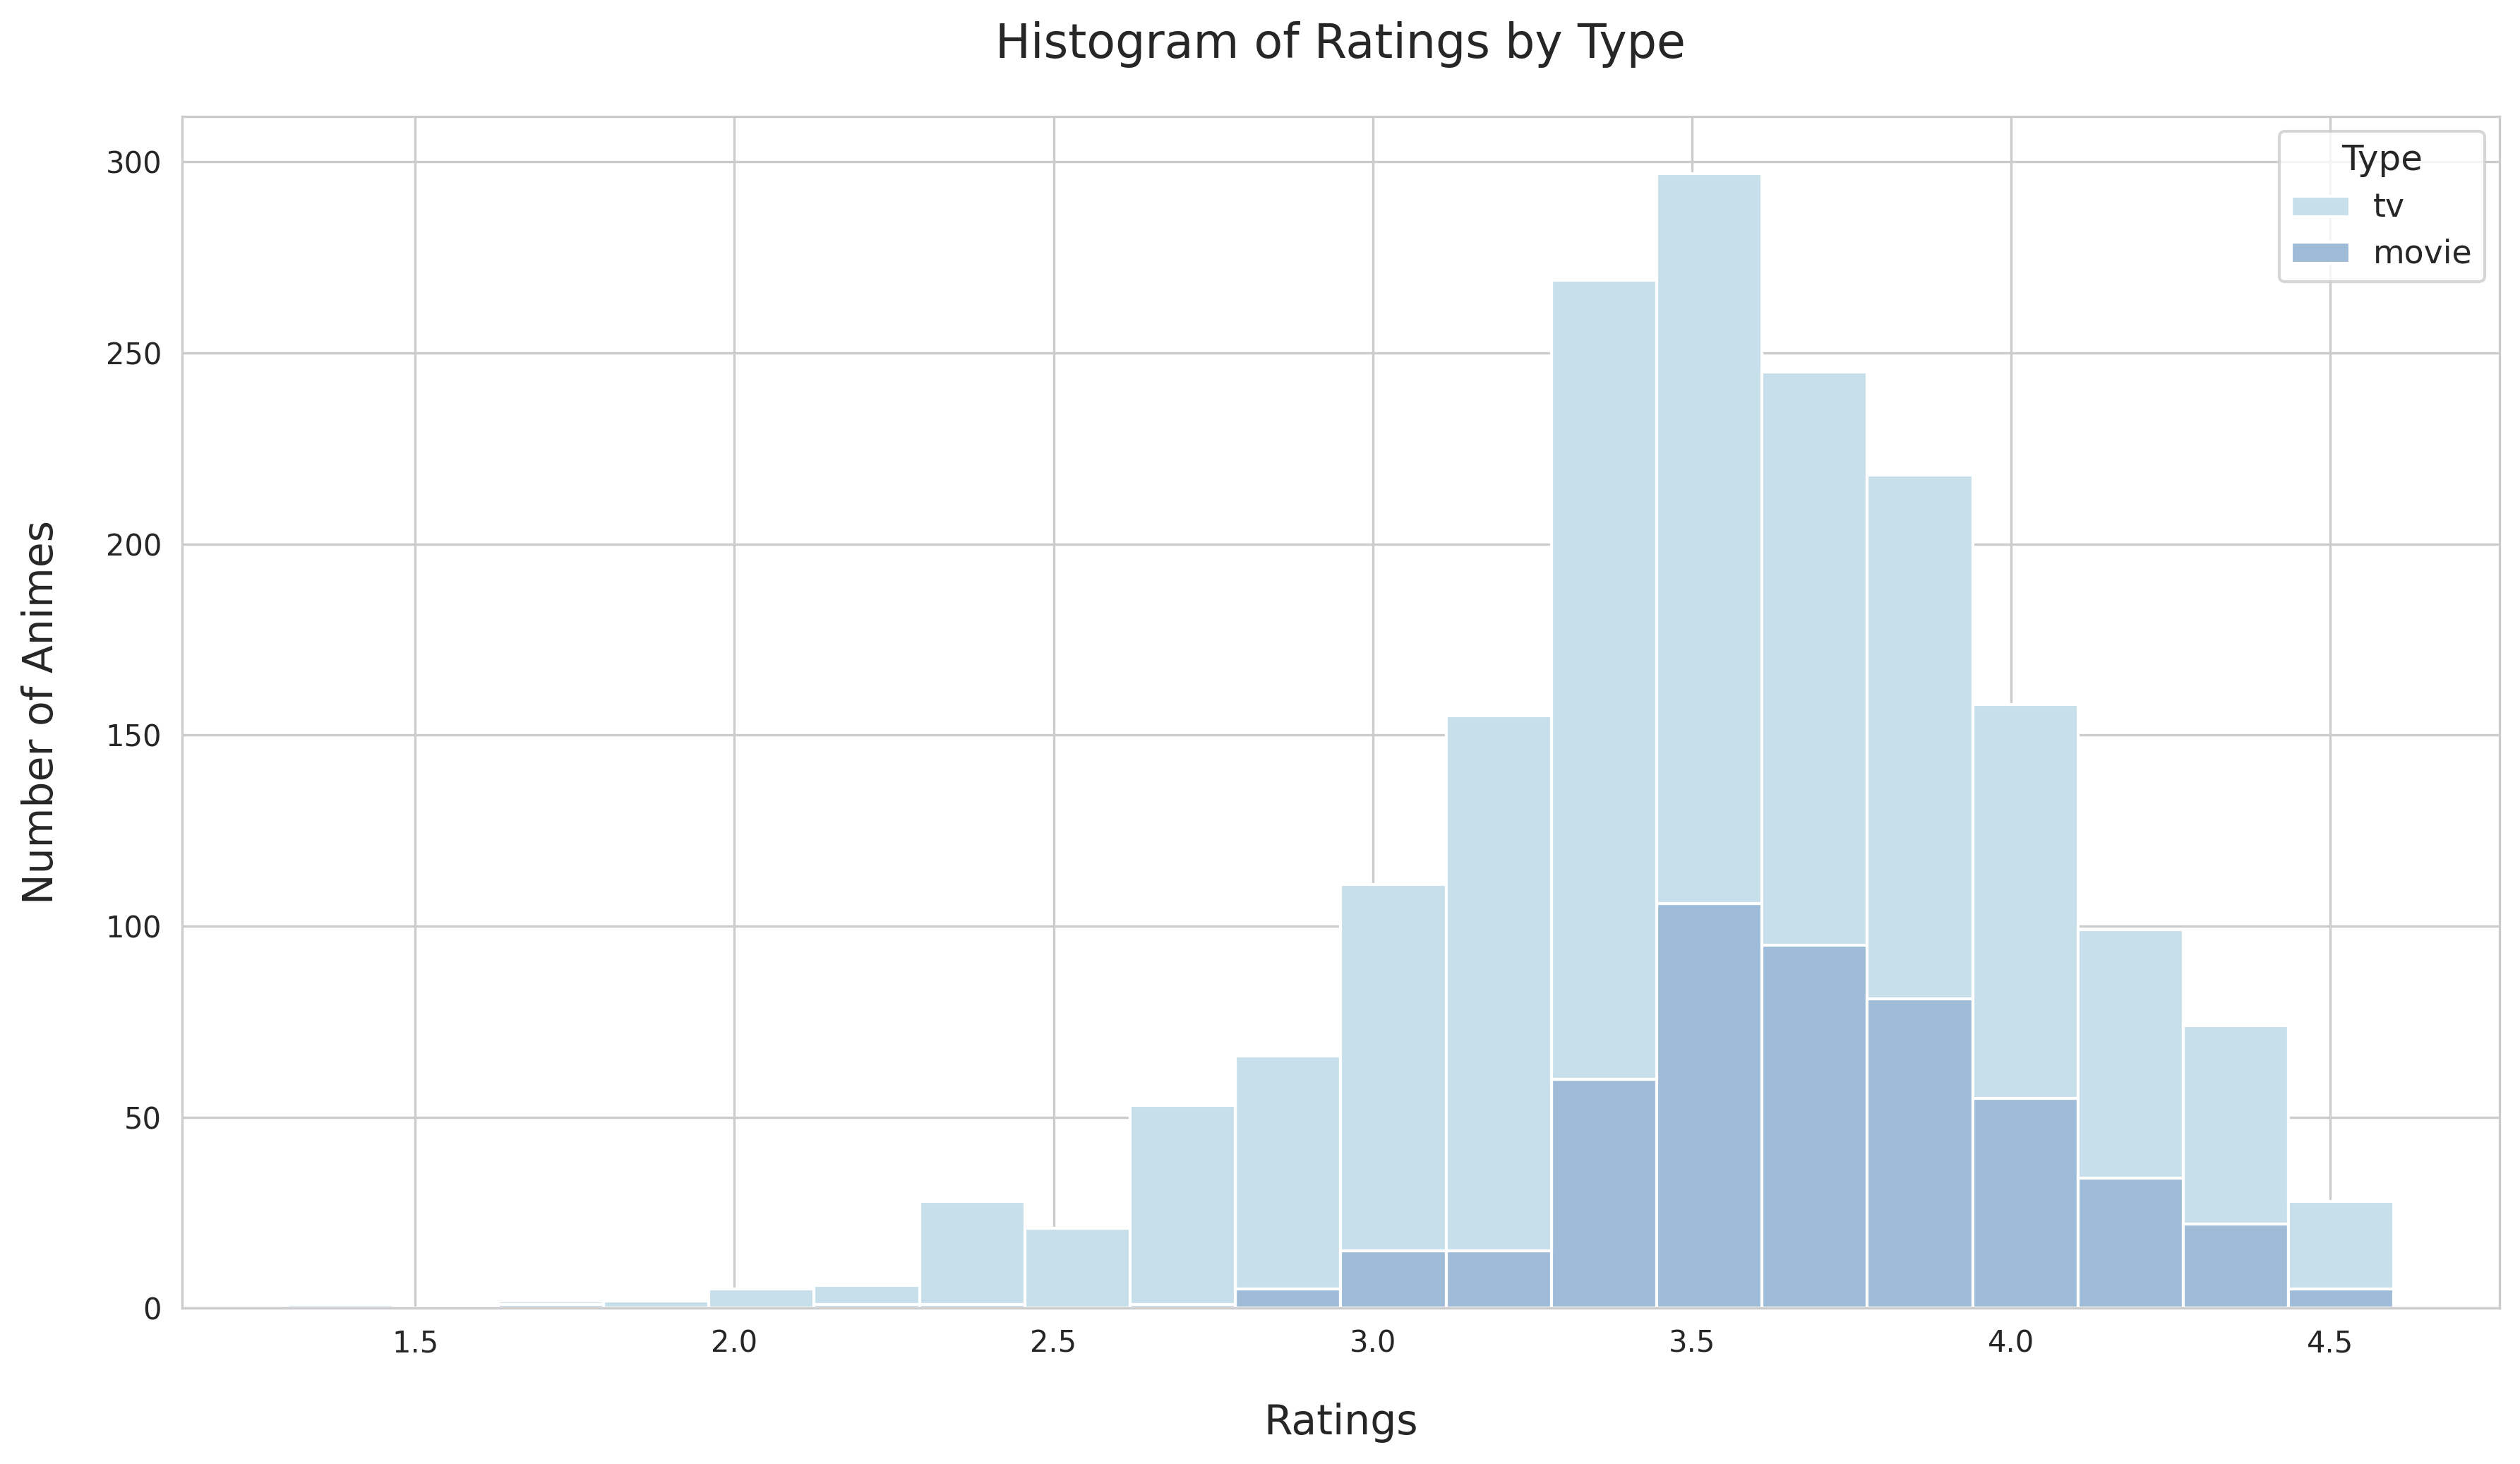
\includegraphics[width=0.95\textwidth]{figures/ratings_by_type_histogram_plot.png}
  
  \textbf{Figure 10:} Histogram of Ratings by Type.
\end{center}
\newpage

\subsection{Part C: Evaluate and Justify Visualization}
For the dataset:
\begin{itemize}
    \item Discuss the advantages and disadvantages of each visualization type.
    \item Decide which visualization is best for the research question.
    \item Support your answer with evidence from the plots and reasoning based on dataset size, shape, or structure.
\end{itemize}
-----\\
